\documentclass[14pt]{extreport}
\usepackage{gost}
\usepackage{amsfonts}

%Тут можно вставить дополнительные пакеты

\begin{document}
\pagestyle{empty} %  выключаем нумерацию

\includepdf[pages=-,pagecommand={}]{Title.pdf}

\pagestyle{plain} % включаем нумерацию
\tableofcontents

\intro

Целью данной работы я поставил «разведку» в область поиска работы в современном мире путём просмотра вакансий на сайте https://spb.hh.ru, а также составления упорядоченной таблицы этих вакансий. Также немаловажной задачей является составление математической страницы с формулами. Вся работа проделана в системе Latex.


\chapter{Математический текст\label{chapter1}}

\section{Числовые множества. Множество действитеьных чисел}

Множества, элементами которых являются числа, называются числовыми. Примерами числовых множеств являются:
\begin{center}
\begin{tabular}{l}
 ${\mathbb {N}}=\{1;2;3;\ldots;{n};\ldots\}$ - множество натуральных чисел; \\ 
 ${\mathbb {Z}_0}=\{0;1;2;\ldots;{n};\ldots\}$ - множество целых неотрицательных чисел; \\  
 ${\mathbb {Z}}=\{0; \pm 1; \pm 2;\ldots;\pm {n};\ldots\}$ - множество целых чисел; \\
 ${\mathbb {Q}}=\{m/n:m \in \mathbb {Z},n \in \mathbb {N}\}$ - множество рациональных чисел. \\
 ${\mathbb {R}}$ - множество действительных чисел. \\
\end{tabular}
\end{center}

Между этими множествами существует соотношение
\[\mathbb {N} \subset \mathbb {Z}_0 \subset \mathbb {Z} \subset \mathbb {Q} \subset \mathbb {R}\eqno(1)\]

Множество R содержит рациональные и иррациональные числа. Всякое рациональное число выражается или конечной десятичной дробью или бесконечной периодической дробью. Так, $\frac{1}{2}=0,5 (=0,500\ldots), \frac{1}{3}=0,333\ldots$ - рациональные числа.

Действительные числа, не являющиеся рациональными, называются иррациональными.
\begin{theorem}

Не существует рационального числа, квадрат которого равен числу 2.
\end{theorem}
\begin{proof}

Допустим, что существует рациональное число, представленное несократимой дробью $\frac{m}{n}$ , квадрат которого равен 2. Тогда имеем:
\[\frac{{m}}{{n}}=2\text{, т.е. }{m}^2=2{n}^2\eqno(2)\]  

Отсюда следует, что $m^2$ (а значит, и $m$) – четное число, т.е. $m=2k$. Подставив $m=2k$ в равенство $m^2=2n^2$, получим $4k^2=2n^2$, т.е. $2k^2=n^2$. Отсюда следует, что число n – четное, т. е $n=2l$. Но тогда дробь $\frac{m}{n}=\frac{2k}{2l}$ сократима. Это противоречит допущению, что $\frac{m}{n}$ дробь несократима. Следовательно, не существует рационального числа, квадрат которого равен числу 2.
\end{proof}
Иррациональное число выражается бесконечной непериодической дробью. Так, $\sqrt(2)=1,4142356\ldots$, $\pi=3,1415926\ldots$ - иррациональные числа. Можно сказать: множество действительных чисел есть множество всех бесконечных десятичных дробей. И записать
\[\mathbb {R}=\{{x}: {x} = {\alpha},{\alpha_1\alpha_2\alpha_3}\ldots\},\text{где }{\alpha} \in \mathbb {Z}, \alpha_i \in \{0,1,\ldots,9\}.\eqno(3)\]

Множество $\mathbb {R}$ действительных чисел обладает следующими свойствами.
\begin{enumerate}
    \item Оно упорядоченное: для любых двух различных чисел $a$ и $b$ имеет место одно из двух соотношений $a<b$ либо $b<a$.
    \item Множество $\mathbb {R}$ плотное: между любыми двумя различными числами $a$ и $b$ содержится бесконечное множество действительных чисел $x$, т.е. чисел, удовлетворяющих неравенству $a<x<b$.
\[({a}<{b} \Rightarrow 2{a}<{a}+{b} \text{ и } {a}+{b}<2{b} \Rightarrow 2{a}<{a}+{b}<2{b} \Rightarrow {a}<\frac{{a}+{b}}{2}<b).\eqno(4)\]
    \item Множество $\mathbb {R}$ непрерывное. Пусть множество $\mathbb {R}$ разбито на два непустых класса $A$ и $B$ таких, что каждое действительное число содержится только в одном классе и для каждой пары чисел $a \in A$ и $b \in B$ выполнено неравенство $a<b$. Тогда (свойство непрерывности) существует единственное число $c$, удовлетворяющее неравенству $a \leqslant c \leqslant b (\forall a \in A, \forall b \in B)$. Оно отделяет числа класса $A$ от чисел класса $B$. Число $c$ является либо наибольшим числом в классе $A$ (тогда в классе $B$ нет наименьшего числа), либо наименьшим числом в классе $B$ (тогда в классе $A$ нет наибольшего).
\end{enumerate}

Свойство неприрывности позволяет установить взаимно-однозначное соответствие между множеством всех действительных чисел и множеством всех точек прямой. Это означает, что каждому числу $x \in \mathbb{R}$ соответствует определенная (единственная) точка числовой оси и, наоборот, каждой точке оси соответствует определенное (единственное) действительное число. Поэтому вместо слова "число" часто говорят "точка".

\section{Числовые промежутки. Окрестность точки}
Пусть $a$ и $b$ - действительные числа, причем $a<b$.
Числовыми промежутками (интервалами) называют подмножества всех действительных чисел, имеющих следующий вид:

\begin{center}
\begin{tabular}{l}
 $[{a};{b}]=\{{x}:{a} \leqslant {x} \leqslant {b} \}$ - отрезок (сегмент, замкнутый промежуток); \\
 $({a};{b})=\{{x}:{a}<{x}<{b}\}$ - интервал (открытый промежуток); \\
 $\text{[}{a};{b})=\{{x}:{a} \leqslant {x}<{b}\}$; \\
 $({a};{b}\text{]}=\{{x}:{a}<{x} \leqslant {b}\}$ - полуоткрытые интервалы (или полуоткрытые отрезки); \\
 $(-\infty;{b}\text{]}=\{{x}:{x} \leqslant {b}\}$;  $\text{[}{a}, +\infty)=\{{x}:{x} \geqslant {a}\}$; \\
 $\text{[}-\infty;{b})=\{{x}:{x}<{b}\}$;  $({a},+\infty)=\{{x}:{x}>a\}$; \\
 $(-\infty;\infty)=\{{x}:-\infty<x<+\infty\}=\mathbb {R}$ - бесконечные интервалы (промежутки). \\
\end{tabular}
\end{center}

Числа $a$ и $b$ называются соответственно левым и правым концами этих промежутков. Символы $-\infty$ и $+\infty$ не числа, это символическое обозначение процесса неограниченного удаления точек числовой оси от начала 0 влево и вправо.
Пусть $x_0$ - любое действительно число (точка на числовой прямой). Окрестностью точки $x_0$ называется любой интервал ($a$;$b$), содержащий точку $x_0$. В частности, интервал ($x_0-\epsilon, x_0+\epsilon$, где $\epsilon>0$, называется $\epsilon$-окрестностью точки $x_0$. Число $x_0$ называется центром, а число $\epsilon$ - радиусом.
\begin{figure}[H]
	\centerline{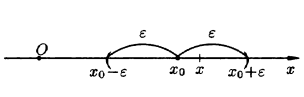
\includegraphics[width=0.5\linewidth]{Окрестность.png}}
	\caption{Окрестность точки $x_0$}
	\label{Окрестность}
\end{figure}
Если $x \in (x_0-\epsilon; x_0+\epsilon)$, то выполняется неравенство $x_0-\epsilon<x<x_0+\epsilon$, или, что то же, $|x-x_0|<\epsilon$. Выполнение последнего неравенства означает попадание точки $x$ в $\epsilon$-окрестность точки $x_0$ (см. рис. 1.1).

\begin{landscape}
\chapter{Таблицы с вакансиями\label{chapter2}}
\begin{table}[H]
	\caption{Web-разработка}\section{Web-разработка}
	\begin{center}
		\begin{small}
		\begin{tabular}{|p{0.1cm}|p{5cm}|p{4.5cm}|p{4.5cm}|p{4cm}|p{3cm}|} \hline
			\multicolumn{1}{|c|}{№}&\multicolumn{1}{c|}{Должность,}&\multicolumn{1}{c|}{Плюсы вакансии}&\multicolumn{1}{c|}{Минусы вакансии}&\multicolumn{1}{c|}{Требования}&\multicolumn{1}{c|}{Дисциплины}\\ 
			\multicolumn{1}{|c|}{п.п.}&\multicolumn{1}{c|}{ссылка, зарплата}&\multicolumn{1}{c|}{}&\multicolumn{1}{c|}{}&\multicolumn{1}{c|}{}&\multicolumn{1}{c|}{из учебного плана}\\ 
			\hline
			1 & Web-разработчик (junior)
			
			\url{https://clck.ru/329fpS}
			
			от 50 000 руб. & 
			• Обучение за счёт компании
			\newline• Опыт работы не требуется
			\newline• Холодильник с кучей еды
			\newline• Мало требований
			&
			• Работа из офиса
			\newline• Начало работы в 9 часов утра
			&
			• Работа с git;
			\newline• Знание PHP от 5.6;
			\newline• Знание JS (jQuery);
			\newline• Разбираться в MySQL
			\newline• Уровень HTML, CSS достаточный для вёрстки с макета.
			&
			Web-программирование, Программирование
			\\
			\hline
			
		\end{tabular}
	\end{small}
	\end{center}
\end{table}



\begin{table}[H]
	\begin{center}
		\begin{small}
		\begin{tabular}{|p{0.1cm}|p{5cm}|p{4.5cm}|p{4.5cm}|p{4cm}|p{3cm}|} \hline
			\multicolumn{1}{|c|}{№}&\multicolumn{1}{c|}{Должность,}&\multicolumn{1}{c|}{Плюсы вакансии}&\multicolumn{1}{c|}{Минусы вакансии}&\multicolumn{1}{c|}{Требования}&\multicolumn{1}{c|}{Дисциплины}\\ 
			\multicolumn{1}{|c|}{п.п.}&\multicolumn{1}{c|}{ссылка, зарплата}&\multicolumn{1}{c|}{}&\multicolumn{1}{c|}{}&\multicolumn{1}{c|}{}&\multicolumn{1}{c|}{из учебного плана}\\ 
			\hline
			    2 & Веб-разработчик
			
    			\url{https://clck.ru/329fsE}
    			
    			~86 000 руб. &
    			• Частично удалённая работа
    			\newline• Обучение за счёт компании
    			\newline• Шаговая доступность от метро
    			\newline• Не много требований
    			&
    			• Начало работы в 9 часов утра
    			\newline• Требуется опыт работы
    			&
    			• Знание HTML, CSS, PHP, MySql, JavaScript, jQuery;
    			\newline• Опыт работы с фреймворками (Laravel, Vue 2), git, *nix системами;
    			\newline• Опыт работы 1-3 года.
    			&
    			Web-программирование, программирование
    			\\
    			\hline
		\end{tabular}
	\end{small}
	\end{center}
\end{table}  
\begin{table}[H]
	\begin{center}
		\begin{small}
		\begin{tabular}{|p{0.1cm}|p{5cm}|p{4.5cm}|p{4.5cm}|p{4cm}|p{3cm}|} \hline
			\multicolumn{1}{|c|}{№}&\multicolumn{1}{c|}{Должность,}&\multicolumn{1}{c|}{Плюсы вакансии}&\multicolumn{1}{c|}{Минусы вакансии}&\multicolumn{1}{c|}{Требования}&\multicolumn{1}{c|}{Дисциплины}\\ 
			\multicolumn{1}{|c|}{п.п.}&\multicolumn{1}{c|}{ссылка, зарплата}&\multicolumn{1}{c|}{}&\multicolumn{1}{c|}{}&\multicolumn{1}{c|}{}&\multicolumn{1}{c|}{из учебного плана}\\ 
			\hline
				3 & Web-программист
				
				\url{https://clck.ru/329fsg}
				от 150 000 руб. &
				• Высокая зарплата
				\newline• Служебная развозка
				\newline• Возможность раскрыть весь свой потенциал, тестировать новые инструменты и сервисы, прокачать аналитические навыки и разработать свои алгоритмы достижения результатов
				&
				• Много требований
				&
				• Опыт работ с Shop-Script, OpenCart
				\newline• HTML5, CSS3, PHP
				\newline• Умение работать с сетками (Bootstrap и т.п.)
				\newline• Кроссбраузерность верстки
				\newline• Умение работать с CSS-препроцессорами (SASS/SCSS, LESS и других)
				\newline• Уверенные знания MySQL
				\newline• Оптимизация кода
				\newline• Опыт работы с API, разработка и интеграция
				\newline• Реализация нового и доработка имеющегося функционала
				&
				Web-программирование, Программирование
				\\ \hline
			\end{tabular}
		\end{small}
	\end{center}
\end{table}
\begin{table}[H]
	\begin{center}
		\begin{small}
		\begin{tabular}{|p{0.1cm}|p{5cm}|p{4.5cm}|p{4.5cm}|p{4cm}|p{3cm}|} \hline
			\multicolumn{1}{|c|}{№}&\multicolumn{1}{c|}{Должность,}&\multicolumn{1}{c|}{Плюсы вакансии}&\multicolumn{1}{c|}{Минусы вакансии}&\multicolumn{1}{c|}{Требования}&\multicolumn{1}{c|}{Дисциплины}\\ 
			\multicolumn{1}{|c|}{п.п.}&\multicolumn{1}{c|}{ссылка, зарплата}&\multicolumn{1}{c|}{}&\multicolumn{1}{c|}{}&\multicolumn{1}{c|}{}&\multicolumn{1}{c|}{из учебного плана}\\ 
			\hline
				4 & Frontend-разработчик
				
				\url{https://clck.ru/329fud}
				до 250 000 руб.
				&
				• Крайне высокая зарплата
				\newline• Дополнительное профильное обучение (за счет компании), с возможностью карьерного роста и повышения заработной платы
				\newline• Гибкий/Удаленный график работы
				\newline• Шаговая доступность от метро
				&
				• Необходимо наличие высшего образования
				\newline• Нет возможности работать дистанционно
				&
				• Высшее образование
				\newline• Опыт разработки на TypeScript
				\newline• Уверенное знание React
				\newline• Опыт работы с React Native
				&
				Web-программирование, Программирование
				\\
				\hline
		\end{tabular}
	\end{small}
	\end{center}
\end{table}
\begin{table}[H]
	\begin{center}
		\begin{small}
		\begin{tabular}{|p{0.1cm}|p{5cm}|p{4.5cm}|p{4.5cm}|p{4cm}|p{3cm}|} \hline
			\multicolumn{1}{|c|}{№}&\multicolumn{1}{c|}{Должность,}&\multicolumn{1}{c|}{Плюсы вакансии}&\multicolumn{1}{c|}{Минусы вакансии}&\multicolumn{1}{c|}{Требования}&\multicolumn{1}{c|}{Дисциплины}\\ 
			\multicolumn{1}{|c|}{п.п.}&\multicolumn{1}{c|}{ссылка, зарплата}&\multicolumn{1}{c|}{}&\multicolumn{1}{c|}{}&\multicolumn{1}{c|}{}&\multicolumn{1}{c|}{из учебного плана}\\ 
			\hline
				5 & Python backend dev
				
				\url{https://clck.ru/328d2E}
				
				150 000 - 250 000 руб. &
				• Удаленная full-time работа и свободный гибкий график, обязательные часы присутствия по будням с 14:00 до 18:00 по Москве
				\newline• Демократичный стиль управления
				\newline• Возможность попробовать себя в сфере инвестиций
				\newline• Высокая зарплата
				&
				• Необходим большой практический опыт работы
				&
				• Опыт работы с SQL / NoSQL базами данных
				\newline• Понимать возможности docker и для чего он нужен
				\newline• Опыт разработки на Python, хорошие теоретические и практические знания
				\newline• Иметь опыт продуктовой разработки
				&
				Проектирование и реализация баз данных, Программирование
				\\
				\hline
				
				
				
			\end{tabular}
		\end{small}
	\end{center}
\end{table}
Вывод: Вакансии в сфере веб-программирования выделяются хорошим соотношением зарплата/требования. К тому же языки программирования, необходимые для устройства на должность, являются относительно простыми в освоении.

\begin{table}[H]
	\caption{Data science}\section{Data science}
	\begin{center}
		\begin{small}
		\begin{tabular}{|p{0.1cm}|p{5cm}|p{4.5cm}|p{4.5cm}|p{4cm}|p{3cm}|} \hline
			\multicolumn{1}{|c|}{№}&\multicolumn{1}{c|}{Должность,}&\multicolumn{1}{c|}{Плюсы вакансии}&\multicolumn{1}{c|}{Минусы вакансии}&\multicolumn{1}{c|}{Требования}&\multicolumn{1}{c|}{Дисциплины}\\ 
			\multicolumn{1}{|c|}{п.п.}&\multicolumn{1}{c|}{ссылка, зарплата}&\multicolumn{1}{c|}{}&\multicolumn{1}{c|}{}&\multicolumn{1}{c|}{}&\multicolumn{1}{c|}{из учебного плана}\\ 
			\hline
				1 & Junior data analyst
				
				\url{https://clck.ru/329gzj}
				
				от 100 000 руб.
				&
				• Большая зарплата
				\newline• Работа в комфортном бизнес-центре на хорошо оборудованном рабочем месте.
				\newline• Удобное местоположение офиса
				\newline• Интересные задачи
				&
				• Нет возможности работать удалённо
				\newline• Необходимо наличие высшего образования
				\newline• Требуется большой практический опыт
				\newline• Много требований
				&
				• Владение Python (в т.ч. библиотеками NumPy, Pandas, scikit-learn)
				\newline• Умение работать с реляционными СУБД, знание SQL
				\newline• Владение базовыми знаниями математической статистики и теории вероятностей на уровне выпускника ВУЗа
				\newline• Системное мышление, аналитический склад ума
				\newline• Высшее образование
				\newline• Опыт работы в анализе данных и/или разработке ПО – от полугода
				\newline• Опыт применения моделей машинного обучения будет пре-
				&
				Матанализ, Дискретная математика, Алгоритмы и структуры данных, Машинное обучение, Проектирование и реализация баз данных, Программирование
				\\
				\hline

					
				\end{tabular}
			\end{small}
		\end{center}
	\end{table}

\begin{table}[H]
	\begin{center}
		\begin{small}
		\begin{tabular}{|p{0.1cm}|p{5cm}|p{4.5cm}|p{4.5cm}|p{4cm}|p{3cm}|} \hline
			\multicolumn{1}{|c|}{№}&\multicolumn{1}{c|}{Должность,}&\multicolumn{1}{c|}{Плюсы вакансии}&\multicolumn{1}{c|}{Минусы вакансии}&\multicolumn{1}{c|}{Требования}&\multicolumn{1}{c|}{Дисциплины}\\ 
			\multicolumn{1}{|c|}{п.п.}&\multicolumn{1}{c|}{ссылка, зарплата}&\multicolumn{1}{c|}{}&\multicolumn{1}{c|}{}&\multicolumn{1}{c|}{}&\multicolumn{1}{c|}{из учебного плана}\\ 
			\hline
			&
			&
			&
			&
			имуществом
			\newline• Опыт работы с BI-инструментами будет преимуществом
			&
			\\
			\hline
			2 & Аналитик DWH
			\newline\url{https://clck.ru/329gzz}
			\newlineНе указана
			&
			• Возможна работа на удалёнке
			\newline• Работа в известной компании (Самокат)
			\newline• ДМС со стоматологией после испытательного срока
			\newline• Возможность участвовать в профильных конференциях в качестве спикера или участника
			&
			• Зарплата не указана
			\newline• Требуется опыт работы
			&
			• Практические навыки применения методологий моделирования данных Data Vault, Dimensional Model
			\newline• Знания в области РСУБД и MPP-систем
			\newline• Отличные знания языка SQL
			\newline• Опыт разработки ETL/ELT приветствуется
			\newline• Опыт работы 1-3 года
			&
			Web-программирование, Матанализ, Дискретная математика, Алгоритмы и структуры данных, Машинное обучение, Проектирование и реализация баз данных
			\\
			\hline
			\end{tabular}
		\end{small}
	\end{center}
\end{table}
			
			

\begin{table}[H]
	\begin{center}
		\begin{small}
		\begin{tabular}{|p{0.1cm}|p{5cm}|p{4.5cm}|p{4.5cm}|p{4cm}|p{3cm}|} \hline
			\multicolumn{1}{|c|}{№}&\multicolumn{1}{c|}{Должность,}&\multicolumn{1}{c|}{Плюсы вакансии}&\multicolumn{1}{c|}{Минусы вакансии}&\multicolumn{1}{c|}{Требования}&\multicolumn{1}{c|}{Дисциплины}\\ 
			\multicolumn{1}{|c|}{п.п.}&\multicolumn{1}{c|}{ссылка, зарплата}&\multicolumn{1}{c|}{}&\multicolumn{1}{c|}{}&\multicolumn{1}{c|}{}&\multicolumn{1}{c|}{из учебного плана}\\ 
			\hline
				3 & Product Analyst
				
				\url{https://clck.ru/329h2i}
				
				2000 - 4000 USD &
				• Выплаты в криптовалюте
				\newline• Европейская компания
				\newline• Можно практиковать английский
				\newline• Работа полностью на удалёнке
				\newline• Крайне высокая зарплата
				&
				Не выявил
				&
				• Опыт работы 1-3 года
				\newline• 1+ лет работы в аналитике
				\newline• Опыт работы над мобильными продуктами или в маркетинге
				\newline• Знание SQL и Python
				\newline• Data Science, cohort, cluster, channel, funnel analytics
				\newline• English(B2+)
				&
				Матанализ, Дискретная математика, Английский язык, Алгоритмы и структуры данных, Мобильные системы передачи данных, Программирование
				\\
				\hline
				
				4 & Data Steward в команду продуктовой аналитики
				
				\url{https://clck.ru/329h37}
				
				Не указана &
				• Работа в VK
				
				• Возможность работы на удалёнке
				
				• Плюшки в виде еды и развлечений (при работе из офиса)
				&
				• Зарплата не указана
				
				• Необходимо наличие высшего образования
				
				• Нужны коммуникативные навыки
				&
				• Опыт работы в Data Governance более 3 лет
				
				• Знание SQL
				
				• Развитые коммуникативные навыки
				
				• Высшее образование в сфере IT, экономики или менеджмента
				&
				Матанализ, Дискретная математика
				\\
			    \hline
			\end{tabular}
		\end{small}
	\end{center}
\end{table}
\begin{table}[H]
	\begin{center}
		\begin{small}
		\begin{tabular}{|p{0.1cm}|p{5cm}|p{4.5cm}|p{4.5cm}|p{4cm}|p{3cm}|} \hline
			\multicolumn{1}{|c|}{№}&\multicolumn{1}{c|}{Должность,}&\multicolumn{1}{c|}{Плюсы вакансии}&\multicolumn{1}{c|}{Минусы вакансии}&\multicolumn{1}{c|}{Требования}&\multicolumn{1}{c|}{Дисциплины}\\ 
			\multicolumn{1}{|c|}{п.п.}&\multicolumn{1}{c|}{ссылка, зарплата}&\multicolumn{1}{c|}{}&\multicolumn{1}{c|}{}&\multicolumn{1}{c|}{}&\multicolumn{1}{c|}{из учебного плана}\\ 
			\hline
			5 & Junior Business Intelligence Analyst
			
			\url{https://clck.ru/329h3N}
			
			1000 - 2000 USD
			&
			• Опыт работы не нужен
			
			• Частичная занятость, удалённая работа
			
			• Возможна подработка
			
			• Международная компания
			
			• Независимость (самоорганизация)
			&
			• Нужен очень высокий уровень английского
			&
			• Английский язык на уровне носителя
			&
			Английский язык, Алгоритмы и структуры данных
			\\
			\hline
			\end{tabular}
		\end{small}
	\end{center}
\end{table}	
Вывод: данные вакансии больше всего сходятся с дисциплинами моего учебного плана. Однако из-за большого количества математики я не вижу своего будущего в направлении data science.
\begin{table}[H]
    \caption{C-программист}\section{C-программист}
	\begin{center}
		\begin{small}
		\begin{tabular}{|p{0.1cm}|p{5cm}|p{4.5cm}|p{4.5cm}|p{4cm}|p{3cm}|} \hline
			\multicolumn{1}{|c|}{№}&\multicolumn{1}{c|}{Должность,}&\multicolumn{1}{c|}{Плюсы вакансии}&\multicolumn{1}{c|}{Минусы вакансии}&\multicolumn{1}{c|}{Требования}&\multicolumn{1}{c|}{Дисциплины}\\ 
			\multicolumn{1}{|c|}{п.п.}&\multicolumn{1}{c|}{ссылка, зарплата}&\multicolumn{1}{c|}{}&\multicolumn{1}{c|}{}&\multicolumn{1}{c|}{}&\multicolumn{1}{c|}{из учебного плана}\\ 
			\hline
				
				1 & Программист-разработчик игр (Junior)
				
				\url{https://clck.ru/329h4L}
				
				1000 - 2000 USD &
				 • Антикризисная система зарплаты
				 
				 • Интересная сфера деятельности
				 
				 • Мало требований
				 &
				 Не выявил
				 &
				 • Иметь базовые знания математики и информационных технологий
				  
				 • Уметь программировать хотя бы на одном из языков: C, C++, Rust
				 &
				 Алгоритмы и структуры данных, Программирование
				\\
				\hline
				2 & Junior C++ Programmer
				
				\url{https://clck.ru/329h4t}
				
				Не указана	&
				 • Расширенный полис ДМС, компенсация спорта и питания
				
				• Релакс-зоны с массажными креслами Yamaguchi и топовыми кофемашинами
				
				• Настольный теннис, хоккей и кикер 
				&
				• Зарплата не указана
				&
				• Хорошие знания C++
				
				• Техническое образование (также студенты последних курсов)
				&
				Алгоритмы и структуры данных, Программирование
				\\
				\hline
			\end{tabular}
		\end{small}
	\end{center}
\end{table}
\begin{table}[H]
	\begin{center}
		\begin{small}
		\begin{tabular}{|p{0.1cm}|p{5cm}|p{4.5cm}|p{4.5cm}|p{4cm}|p{3cm}|} \hline
			\multicolumn{1}{|c|}{№}&\multicolumn{1}{c|}{Должность,}&\multicolumn{1}{c|}{Плюсы вакансии}&\multicolumn{1}{c|}{Минусы вакансии}&\multicolumn{1}{c|}{Требования}&\multicolumn{1}{c|}{Дисциплины}\\ 
			\multicolumn{1}{|c|}{п.п.}&\multicolumn{1}{c|}{ссылка, зарплата}&\multicolumn{1}{c|}{}&\multicolumn{1}{c|}{}&\multicolumn{1}{c|}{}&\multicolumn{1}{c|}{из учебного плана}\\ 
			\hline				
				3 & Программист C\#
				
				\url{https://clck.ru/329h4t}
				
				Не указана	&
				• Полностью удалённая работа (40ч в неделю)
				
				• Оплачиваемый отпуск и больничные
				
				• Международная компания
				
				• Не много требований 
				&
				• Зарплата не указана
				
				• Требуется опыт работы 
				&
				• Понимание сложности алгоритмов, O-нотация
				
				• Опыт коммерческой разработки с использованием .NET/C\#
				
				• Способность писать чистый, понятный и поддерживаемый код
				
				• Знание английского языка
				
				• Умение разбираться в чужом коде и улучшать его
				
				• Опыт работы 1-3 года 
				&
				Алгоритмы и структуры данных, Английский язык, Программирование
				\\
				\hline
			\end{tabular}
		\end{small}
	\end{center}
\end{table}

\begin{table}[H]
	\begin{center}
		\begin{small}
		\begin{tabular}{|p{0.1cm}|p{5cm}|p{4.5cm}|p{4.5cm}|p{4cm}|p{3cm}|} \hline
			\multicolumn{1}{|c|}{№}&\multicolumn{1}{c|}{Должность,}&\multicolumn{1}{c|}{Плюсы вакансии}&\multicolumn{1}{c|}{Минусы вакансии}&\multicolumn{1}{c|}{Требования}&\multicolumn{1}{c|}{Дисциплины}\\ 
			\multicolumn{1}{|c|}{п.п.}&\multicolumn{1}{c|}{ссылка, зарплата}&\multicolumn{1}{c|}{}&\multicolumn{1}{c|}{}&\multicolumn{1}{c|}{}&\multicolumn{1}{c|}{из учебного плана}\\ 
			\hline		
				4 & Программист С\# (.Net Developer)
				
				\url{https://clck.ru/329h5J}
				
				100 000 - 150 000 руб. &
				• Международная компания
				
				• Большая зарплата
				
				• Интересный мне язык программирования
				&
				• Требуется опыт работы
				&
				• Знание C\#‚ .Net Framework
				 
				• Базовые знания SQL, опыт работы с MSSQL
				
				• знание основных концепций ООП и паттернов проектирования
				
				• Владение многопоточным программированием
				
				• знание английского на уровне чтения технической документации
				
				• Опыт работы 1-3 года 
				&
				Алгоритмы и структуры данных, Объектно-ориентированное программирование, Программирование
				\\
				\hline
			\end{tabular}
		\end{small}
	\end{center}
\end{table}
\begin{table}[H]
	\begin{center}
		\begin{small}
		\begin{tabular}{|p{0.1cm}|p{5cm}|p{4.5cm}|p{4.5cm}|p{4cm}|p{3cm}|} \hline
			\multicolumn{1}{|c|}{№}&\multicolumn{1}{c|}{Должность,}&\multicolumn{1}{c|}{Плюсы вакансии}&\multicolumn{1}{c|}{Минусы вакансии}&\multicolumn{1}{c|}{Требования}&\multicolumn{1}{c|}{Дисциплины}\\ 
			\multicolumn{1}{|c|}{п.п.}&\multicolumn{1}{c|}{ссылка, зарплата}&\multicolumn{1}{c|}{}&\multicolumn{1}{c|}{}&\multicolumn{1}{c|}{}&\multicolumn{1}{c|}{из учебного плана}\\ 
			\hline	
			5 & PHP программист
				
			\url{https://clck.ru/329h5c}
			
			100 000 - 150 000 руб. &
			• "Если вы не обладаете базовыми компетенциями (знание CMS 1C-Битрикс, Битрикс24, базовое системное администрирование) - это не является проблемой и мы обеспечим для Вас возможность обучения."
			
			• Работа на удалёнке
			&
			• Требуется опыт работы
			&
			• Наличие не менее 3х скиллов из списка: PHP, HTML5, CSS3, Javascript, MySql
			
			• Опыт работы 1-3 года
			&
			Web-программирование, Программирование
			\\
			\hline
			\end{tabular}
		\end{small}
	\end{center}
\end{table}			
Вывод: данные вакансии заинтересовали меня больше всего, так как мне нравится программировать и составлять алгоритмы. Языки программирования C\# и C++ также являются для меня несомненным плюсом.
\end{landscape}

\conclusions

Работа выполнена, так как я проанализировал вакансии, упорядочил их в таблице и извлёк для себя пользу, ведь теперь я имею хотя бы примерное представление о состоянии рынка труда в заинтересовавших меня сферах IT. С помощью проделанной работы я познакомился с Latex и научился пользоваться этой системой.

% Оформляем библиографию в соответствии с ГОСТ 7.0.5
% \bibliographystyle{ugost2008}
% если хотим включить все источники из библиографии даже не имеющие ссылки из текта
% \nocite{*}
% файл с библиографией
% \bibliography{biblio.bib}

\newpage
\begin{thebibliography}{99}
\bibitem{bib1} HeadHunter : официальный сайт. [Электронный ресурс]: [сайт]. - URL: \url{https://spb.hh.ru} (дата обращения: 18.09.2022). - Загл. с экрана. - Яз.рус.

\bibitem{bib2} Письменный, Д. Т. Конспект лекций по высшей математике: полный курс / Д. Т. Письменный. – 10-е изд., испр. – М.: Айрис-пресс, 2011. – 608 с.: ил. – (Высшее образование).
\end{thebibliography}


\Appendix % Приложения

\chapter{Рисунки математического текста}

\begin{figure}[H]
	\centerline{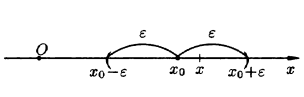
\includegraphics[width=0.5\linewidth]{Окрестность.png}}
	\caption{Окрестность точки $x_0$}
	\label{Окрестность}
\end{figure}

\end{document}
